\section[Monthly TVAR Impulse Response Atlas (1960--1980)]{Atlas of High-Frequency Monthly TVAR Impulse Responses\\Across Solvency Regimes (1960--1980)}
\label{app:annual_tvar}
\label{app:tvar_girf_atlas}

To evaluate the non-linear macroeconomic transmission mechanism under balance-sheet exhaustion without temporal aggregation distortions, this appendix presents the comprehensive Generalized Impulse Response Function (GIRF) atlas across sixty dynamic trajectories. The empirical system comprises the four-variable endogenous monthly vector ($N=252$, 1960:01--1980:12):
\begin{equation}
y_t = \big[ g_{P,\text{gold},t},\; \Delta \ln \Theta_t,\; \Delta \pi_t,\; \Delta g_{H,t} \big]'
\label{eq:app_c_tvar_system}
\end{equation}
conditioned on lagged Central Bank reserve solvency $\text{SolvR}_{t-1} \equiv \frac{e_{t-1} \cdot IR_{t-1}}{M1_{t-1}}$ across the three Minskian solvency regimes: Hedge ($\text{SolvR} > 0.21$), Speculative ($0.14 < \text{SolvR} \le 0.21$), and Forced Ponzi ($\text{SolvR} \le 0.14$).

All impulse responses are computed via the nested two-loop simulation algorithm synthesized from \citet{KoopPesaranPotter1996}, \citet{Balke2000}, and \citet{Afonso2018}:
\begin{enumerate}[leftmargin=2em]
	\item \textbf{Parameter Uncertainty (Outer Loop):} $B = 500$ stratified residual bootstrap replications are executed, drawing residuals independently from each regime's empirical residual covariance matrix $\hat{\Sigma}_k$ to preserve regime-specific conditional heteroskedasticity \citep{GoncalvesKilian2004}.
	\item \textbf{History-Conditioned Shock Propagation (Inner Loop):} For each historical starting month $t_0 \in \mathcal{T}_k$, orthogonalized Cholesky structural innovations $v_0 = P_k e_j$ are propagated forward over $h = 0, \dots, 8$ months along the empirical regime sequence.
	\item \textbf{Credibility Ribbons:} Following \citet{SimsZha1999} and \citet{RodriguezAsensio2026}, each panel displays the empirical median trajectory (solid line), the primary 68\% confidence ribbon (16th--84th percentiles, darker shading), and the 95\% conservative bounds (2.5th--97.5th percentiles, lighter shading), evaluated against the neutral grey horizontal zero reference line.
\end{enumerate}

\begin{figure}[H]
\centering
\caption{Master Nonlinear Generalized Impulse Response Matrix: Real Structural Imbalance, Base Money, and Inflation Across Minskian Solvency Regimes}
\label{fig:girf_regimes_matrix}
\label{fig:app_c00_master_3x3}
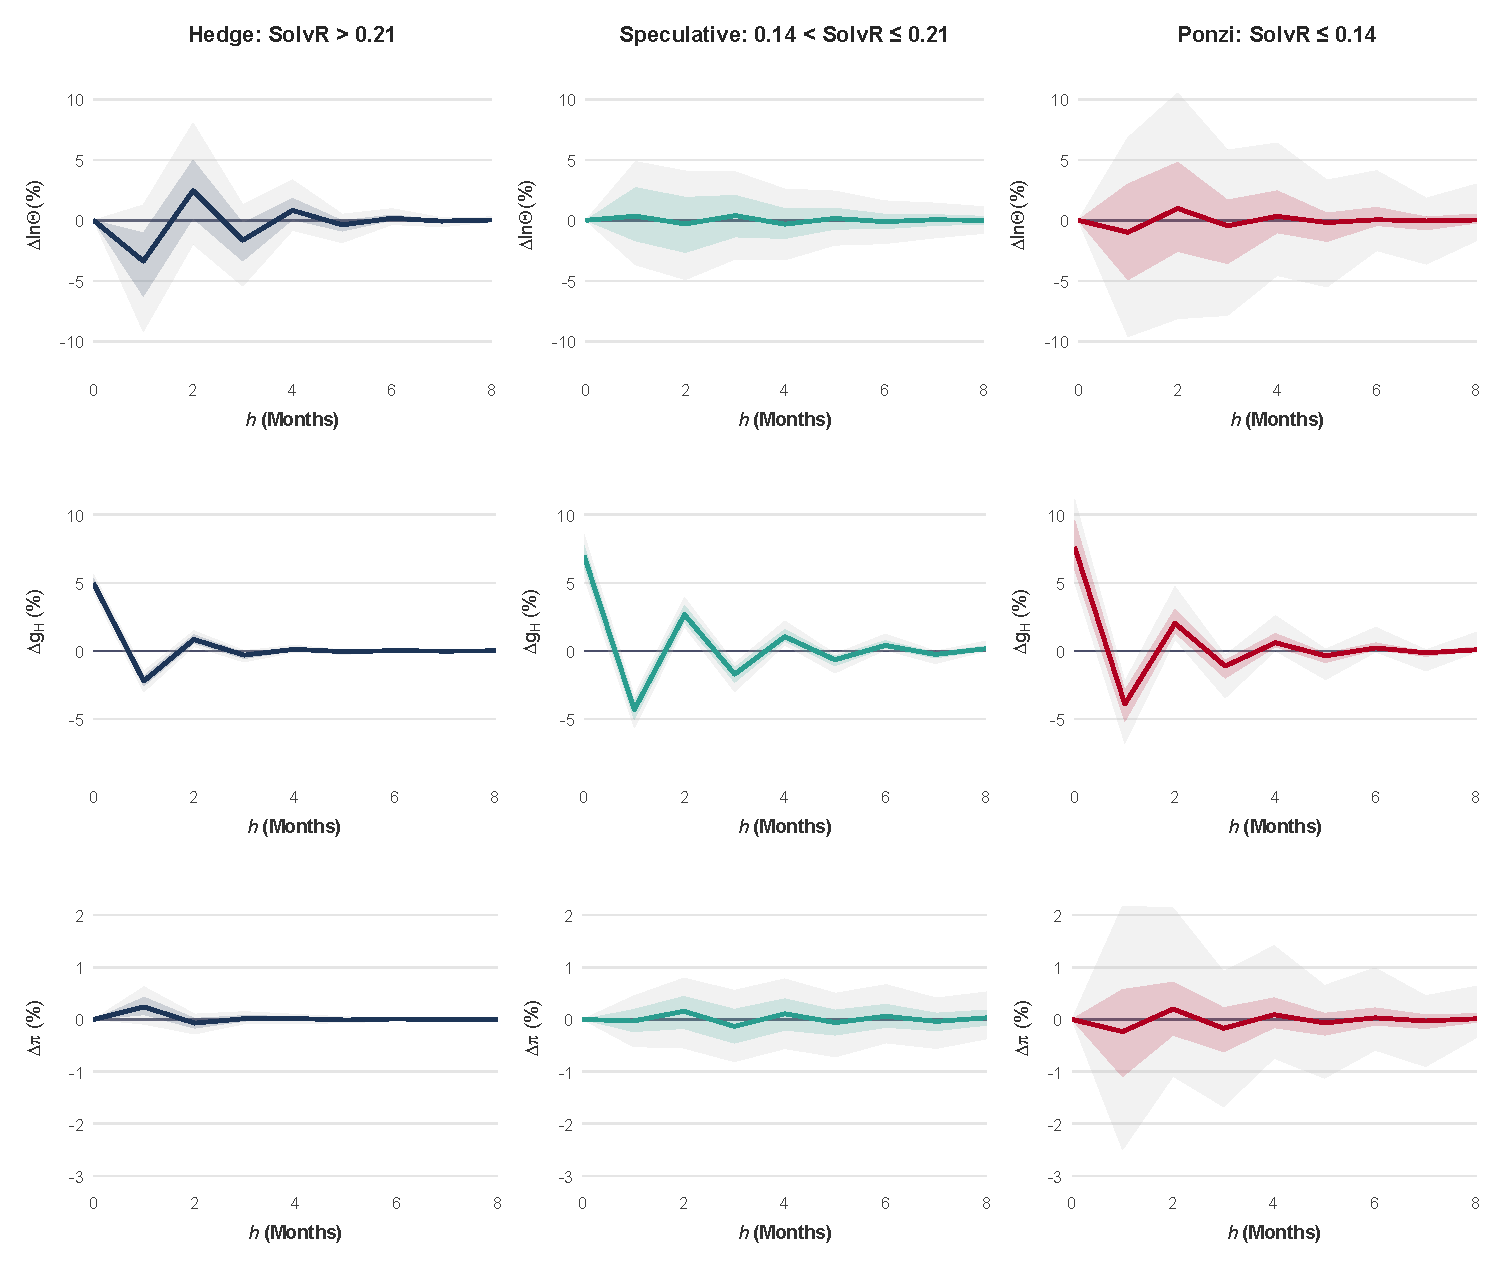
\includegraphics[width=\textwidth]{figures/fig04_tvar_girf_inflation.pdf}
\begin{tabular}{p{0.95\textwidth}}
\footnotesize \textbf{Notes:} Generalized Impulse Response Functions (GIRFs) of the Real Structural Imbalance ($\Delta \ln \Theta_t$), base money growth ($\Delta g_{H,t}$), and consumer price inflation ($\Delta \pi_t$) to a $+1\sigma$ orthogonalized base money expansion shock ($\Delta g_H$), estimated from a 3-regime TVAR(1) with predetermined delay $d=1$ ($\text{SolvR}_{t-1}$). Structural identification follows the recursive Cholesky ordering vector $[g_{P,\text{gold},t}, \Delta \ln \Theta_t, \Delta \pi_t, \Delta g_{H,t}]'$ certified non-parametrically by the PCMCI contemporaneous DAG (Appendix~\ref{app:causal_pcmci}). Solid colored lines display empirical median responses across Minskyan postures (navy for Hedge, teal for Speculative, crimson for Forced Ponzi); darker and lighter shaded polygons display 68\% and 95\% stratified residual bootstrap credibility bands ($B=500$ replications) following \citet{SimsZha1999} and \citet{RodriguezAsensio2026}, evaluated against the neutral grey horizontal zero reference line over horizon $h=8$ months. Responses are expressed in percentage-point monthly deviations. Data sources: Central Bank of Chile (BCCh), INE, and London Bullion Market (1960:01--1980:12, $N=250$). Complete $4 \times 4$ regime response matrices covering all 48 shock-response combinations are documented in Figures~\ref{fig:app_c01_hedge}--\ref{fig:app_c05_scissors_atlas}.
\end{tabular}
\end{figure}

\begin{figure}[H]
\centering
\caption{Full $4 \times 4$ Impulse Response Matrix: Hedge Regime ($\text{SolvR} > 0.21$)}
\label{fig:app_c01_hedge}
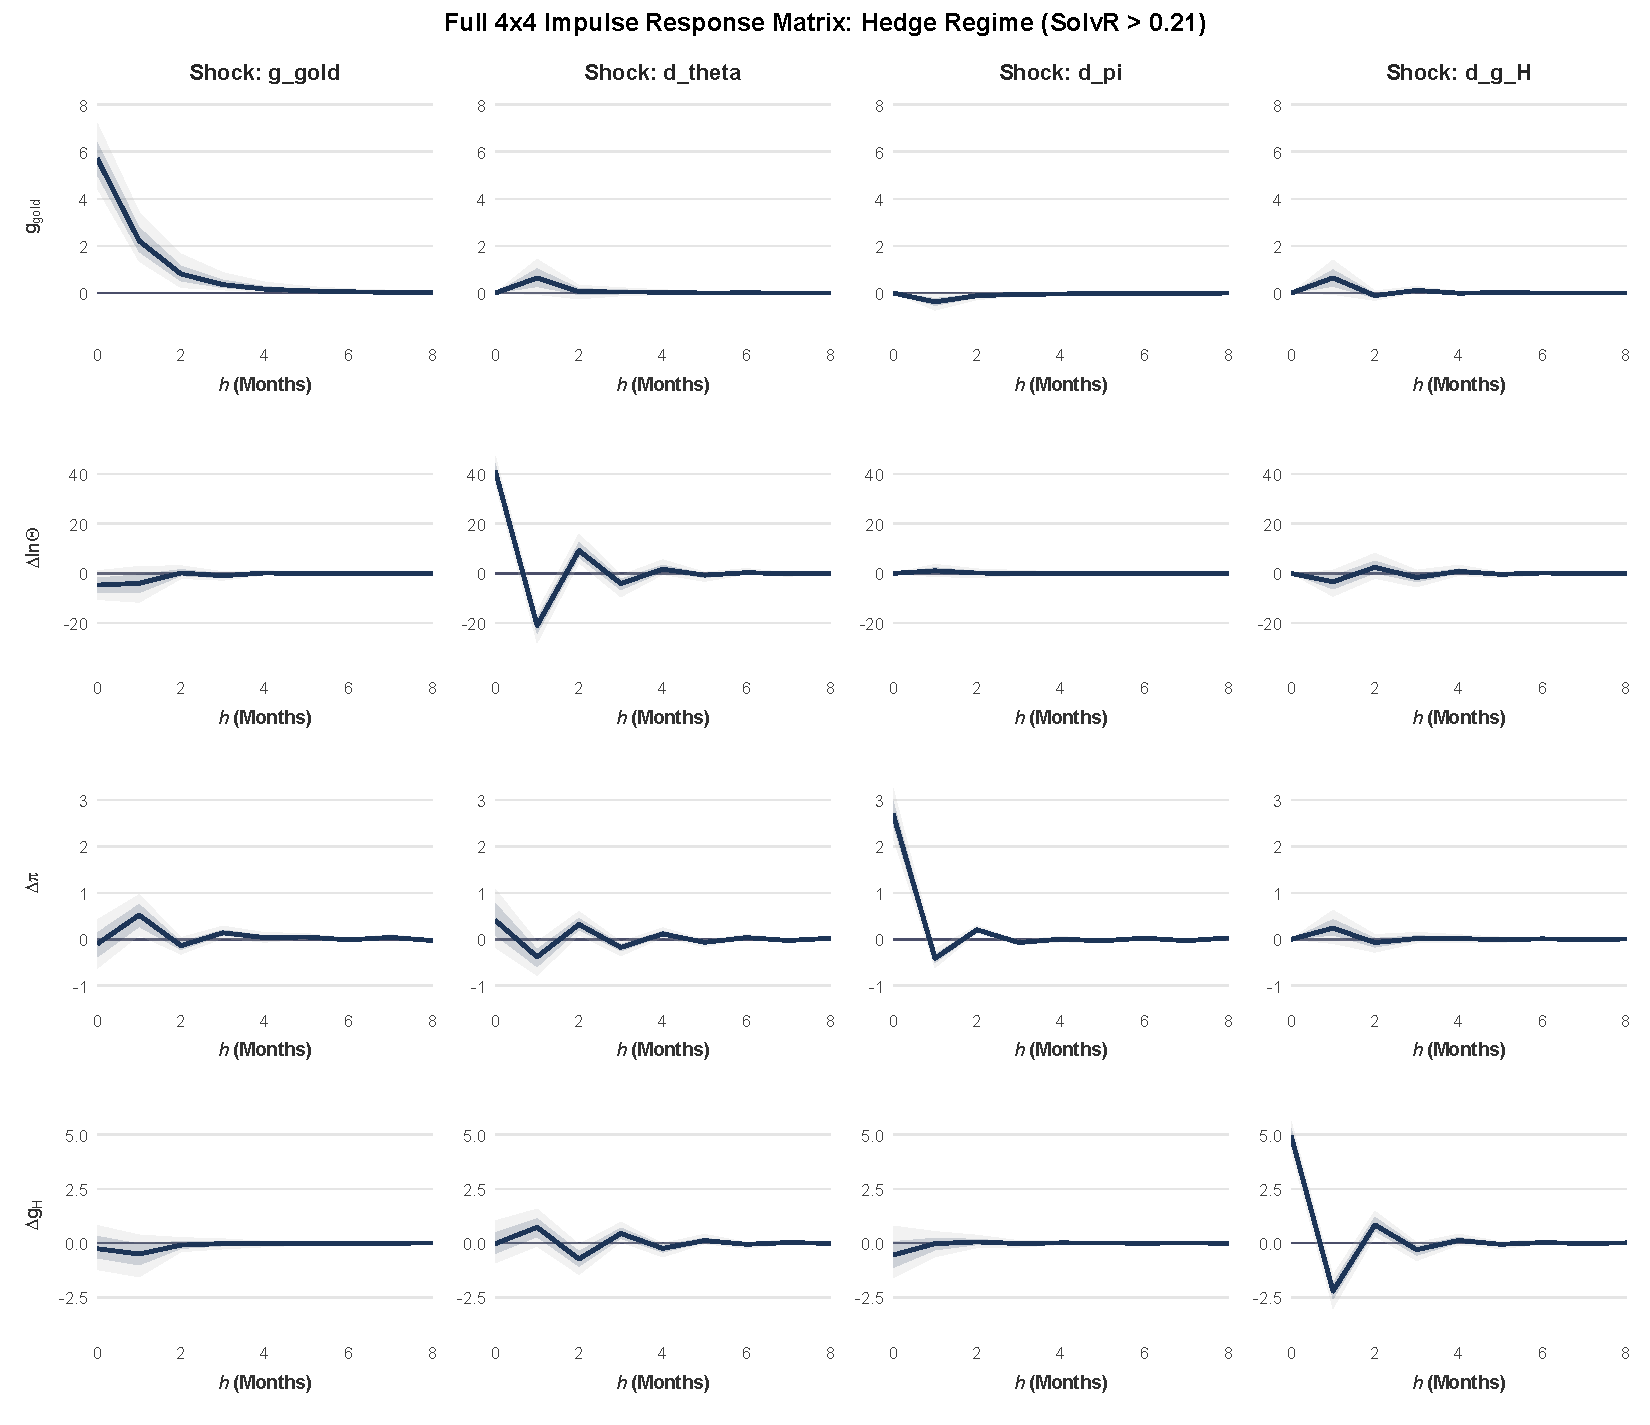
\includegraphics[width=0.92\textwidth]{figures/fig_app_c01_hedge_4x4.pdf}
\begin{tabular}{p{0.95\textwidth}}
\footnotesize \textbf{Notes:} Complete 16-panel Generalized Impulse Response Function (GIRF) matrix for the Hedge regime ($\text{SolvR}_{t-1} > 0.21$, $N=143$ months) from the 3-regime TVAR(1) with predetermined delay $d=1$. Columns indicate $+1\sigma$ orthogonalized structural shocks; rows denote endogenous response variables ($g_{P,\text{gold}}, \Delta \ln \Theta, \Delta \pi, \Delta g_H$). Identification follows the Cholesky vector $[g_{P,\text{gold},t}, \Delta \ln \Theta_t, \Delta \pi_t, \Delta g_{H,t}]'$ authorized by the PCMCI DAG. Trajectories trace horizons $h=0\dots 8$ months; shaded bands represent 68\% (darker) and 95\% (lighter) stratified residual bootstrap credibility bands ($B=500$). Responses are measured in percentage-point monthly deviations. Under anchored external solvency, base money shocks (Column 4) produce statistically zero price acceleration. Data sources: Central Bank of Chile (BCCh), INE, and London Bullion Market (1960:01--1980:12).
\end{tabular}
\end{figure}

\begin{figure}[H]
\centering
\caption{Full $4 \times 4$ Impulse Response Matrix: Speculative Regime ($0.14 < \text{SolvR} \le 0.21$)}
\label{fig:app_c02_spec}
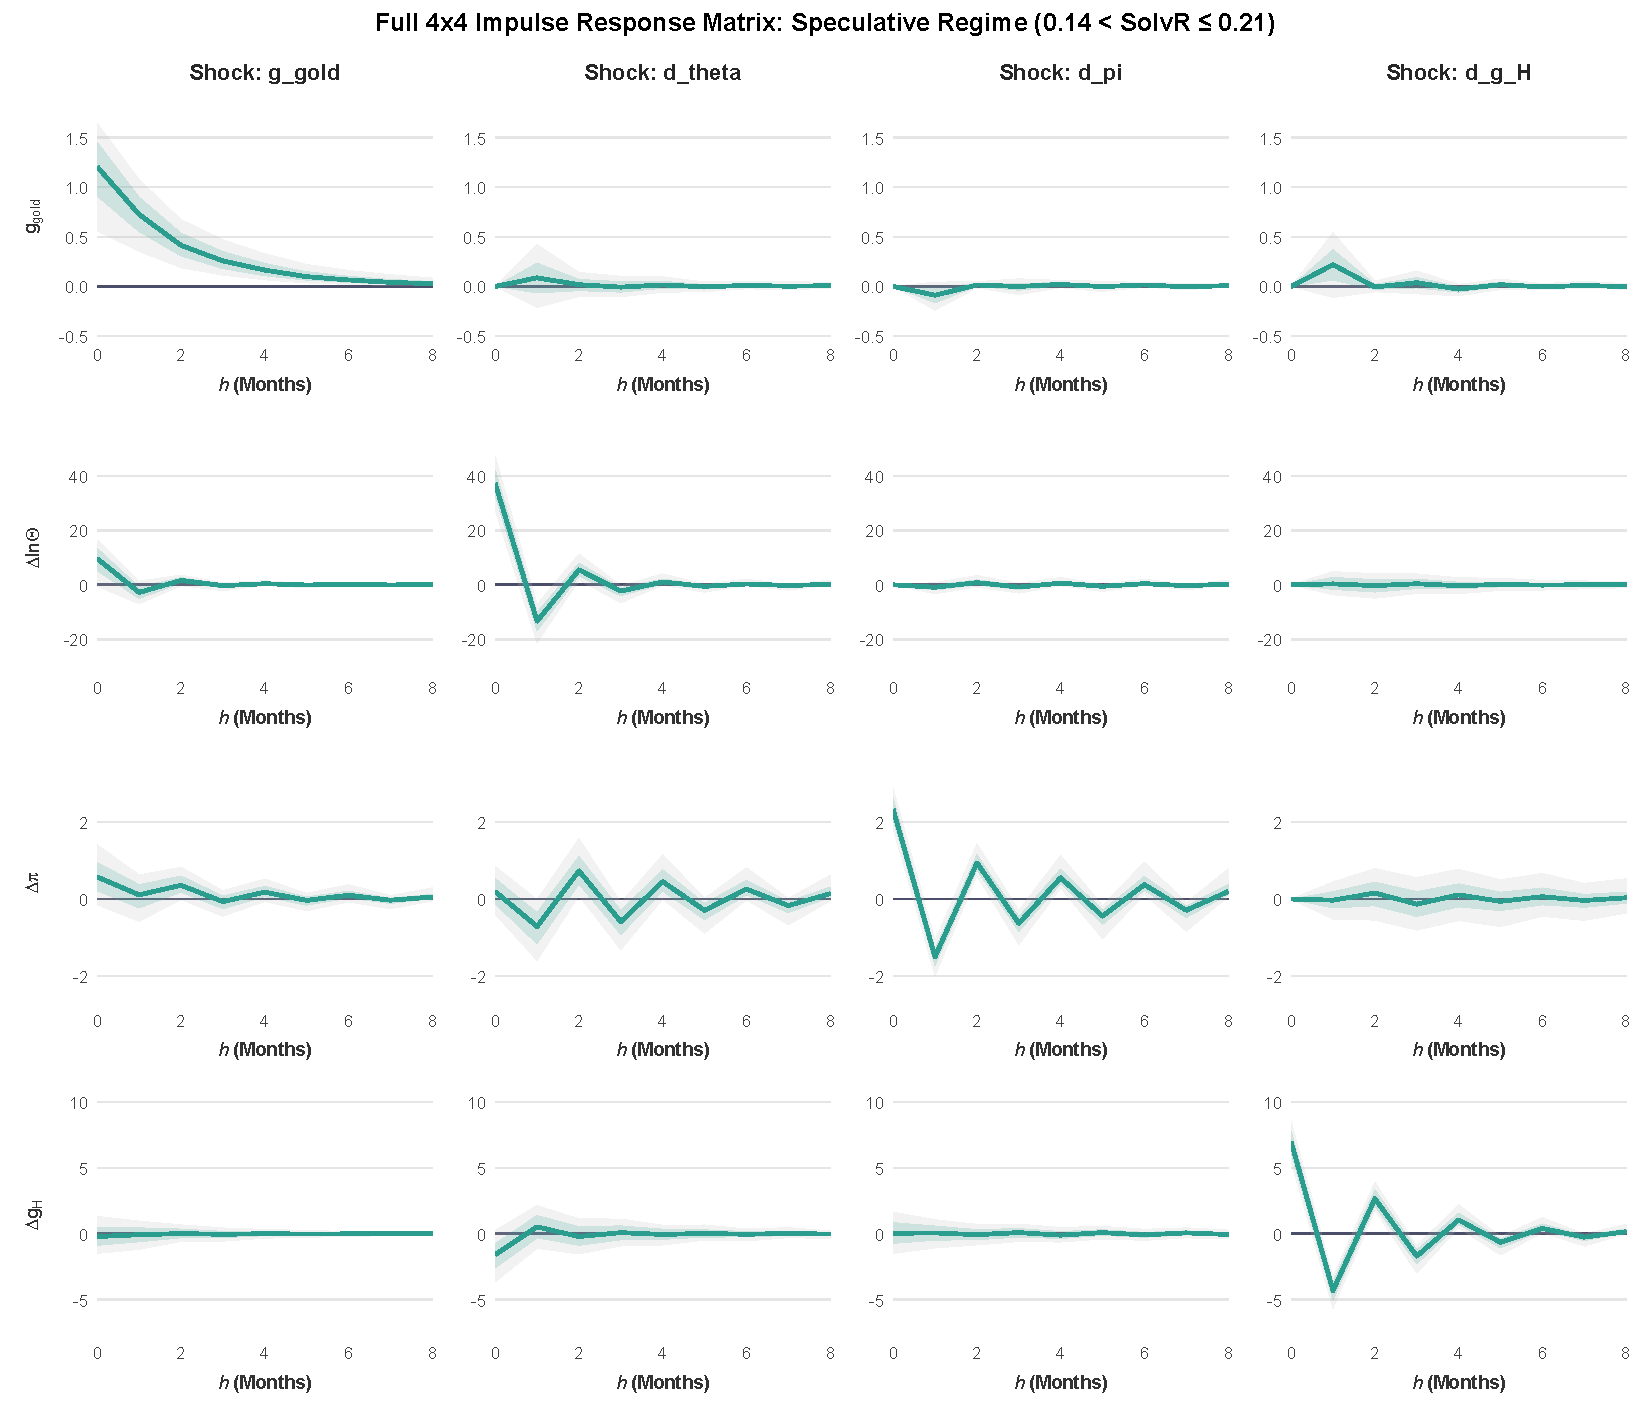
\includegraphics[width=0.92\textwidth]{figures/fig_app_c02_spec_4x4.pdf}
\begin{tabular}{p{0.95\textwidth}}
\footnotesize \textbf{Notes:} Complete 16-panel Generalized Impulse Response Function (GIRF) matrix for the Speculative regime ($0.14 < \text{SolvR}_{t-1} \le 0.21$, $N=62$ months) from the 3-regime TVAR(1) with predetermined delay $d=1$. Columns indicate $+1\sigma$ orthogonalized structural shocks; rows denote endogenous responses. Structural identification follows the recursive Cholesky ordering vector $[g_{P,\text{gold},t}, \Delta \ln \Theta_t, \Delta \pi_t, \Delta g_{H,t}]'$ certified by the PCMCI DAG. Shaded ribbons depict 68\% and 95\% stratified residual bootstrap credibility bands ($B=500$ replications) over horizon $h=0\dots 8$ months, evaluated against the neutral grey horizontal zero reference line. Responses are in percentage-point monthly deviations. As foreign reserve coverage erodes, external gold price shocks (Column 1) pass violently into domestic inflation. Data sources: Central Bank of Chile (BCCh), INE, and London Bullion Market (1960:01--1980:12).
\end{tabular}
\end{figure}

\begin{figure}[H]
\centering
\caption{Full $4 \times 4$ Impulse Response Matrix: Forced Ponzi Regime ($\text{SolvR} \le 0.14$)}
\label{fig:app_c03_ponzi}
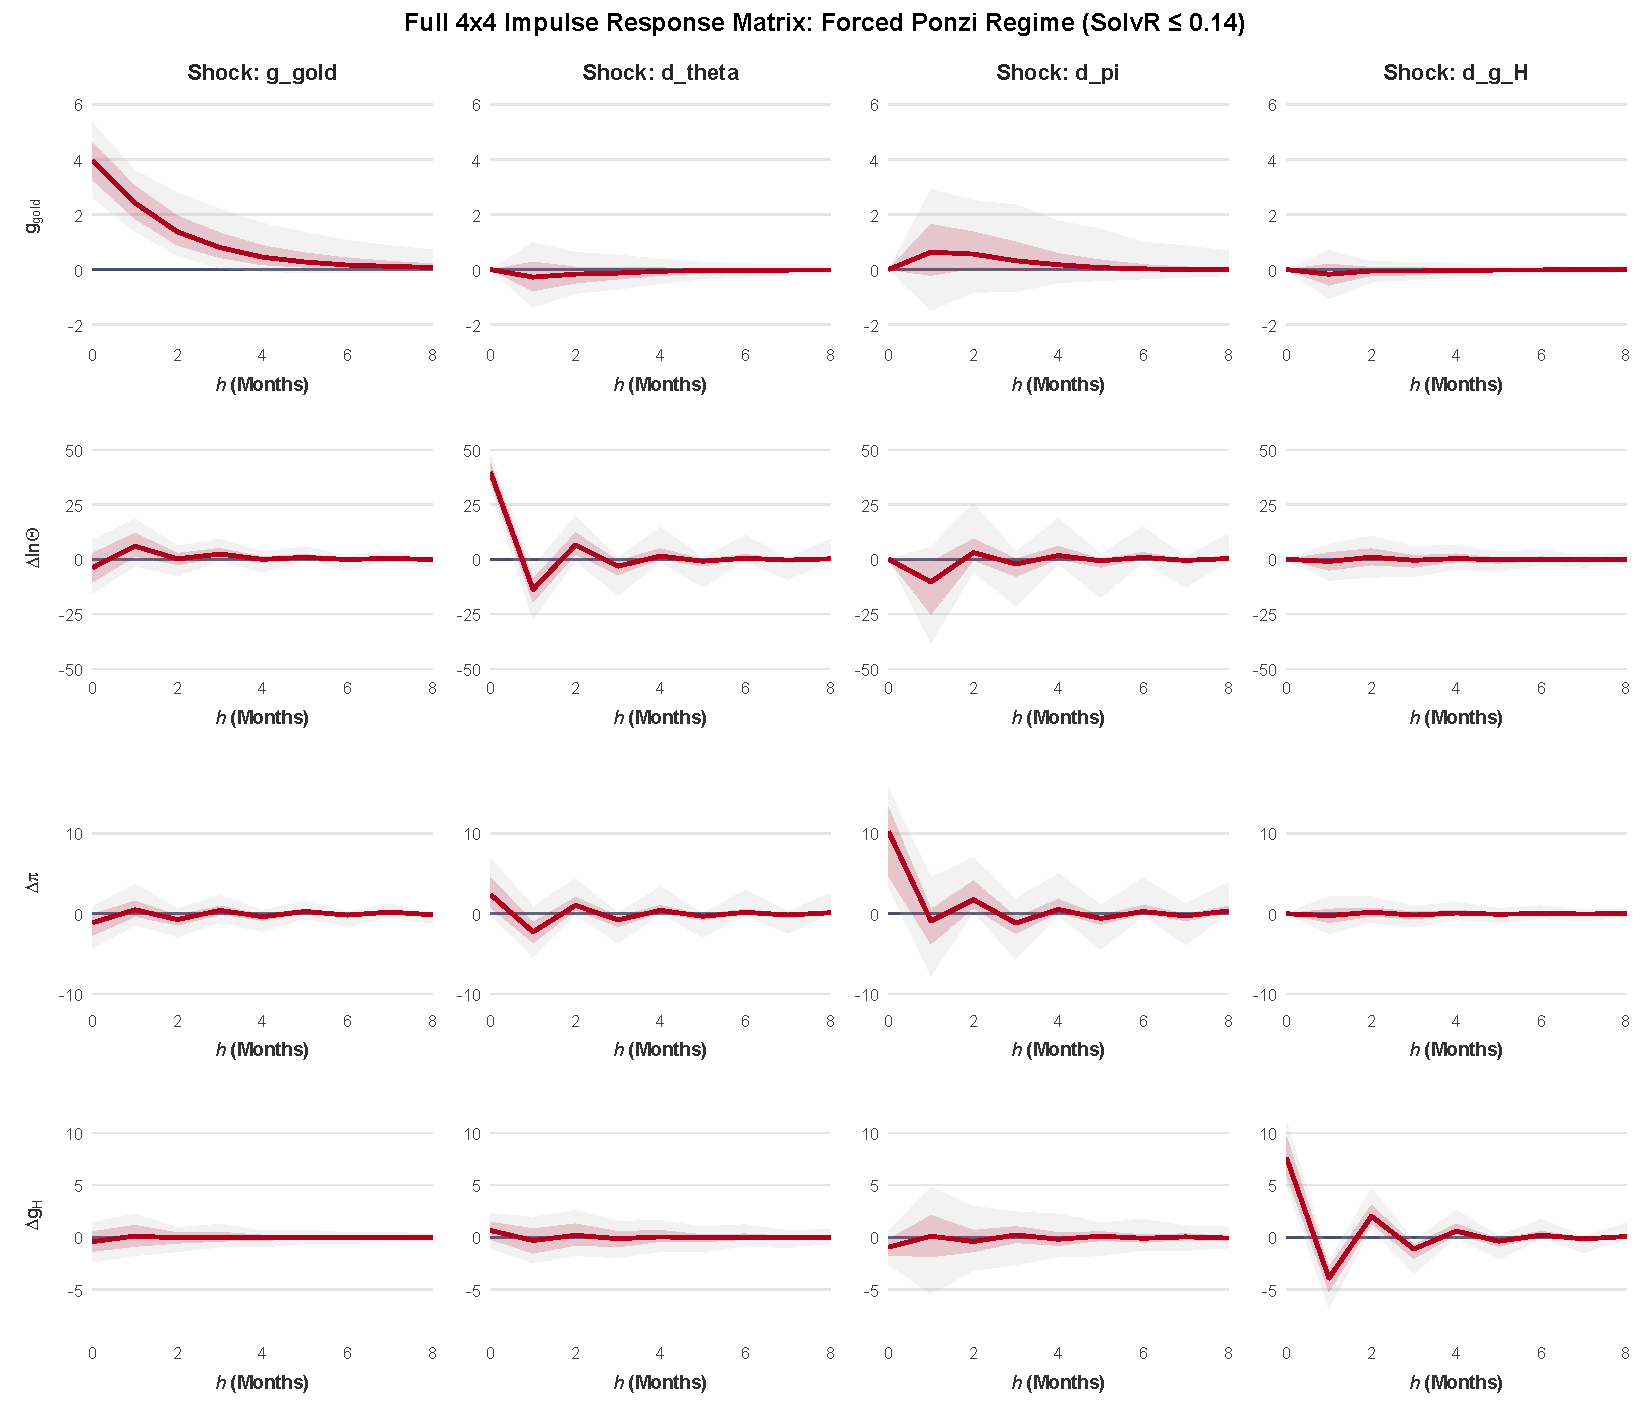
\includegraphics[width=0.92\textwidth]{figures/fig_app_c03_ponzi_4x4.pdf}
\begin{tabular}{p{0.95\textwidth}}
\footnotesize \textbf{Notes:} Complete 16-panel Generalized Impulse Response Function (GIRF) matrix for the Forced Ponzi regime ($\text{SolvR}_{t-1} \le 0.14$, $N=45$ months) from the 3-regime TVAR(1) with predetermined delay $d=1$. Columns indicate $+1\sigma$ orthogonalized structural shocks; rows denote endogenous responses. Structural identification follows the recursive Cholesky vector $[g_{P,\text{gold},t}, \Delta \ln \Theta_t, \Delta \pi_t, \Delta g_{H,t}]'$ certified by the PCMCI DAG. Shaded ribbons depict 68\% and 95\% stratified residual bootstrap credibility bands ($B=500$) across $h=0\dots 8$ months, evaluated against the neutral grey horizontal zero reference line. Responses are in percentage-point monthly deviations. Under liquid reserve exhaustion, domestic inflation shocks (Column 3) trigger immediate, persistent defensive base money accommodation (Row 4), while monetary shocks (Column 4) unleash explosive price acceleration. Data sources: Central Bank of Chile (BCCh), INE, and London Bullion Market (1960:01--1980:12).
\end{tabular}
\end{figure}

\begin{figure}[H]
\centering
\caption{Cross-Regime Transmission Atlas: Nixon Shock and World Gold Price Growth ($g_{P,\text{gold}}$)}
\label{fig:app_c04_gold_atlas}
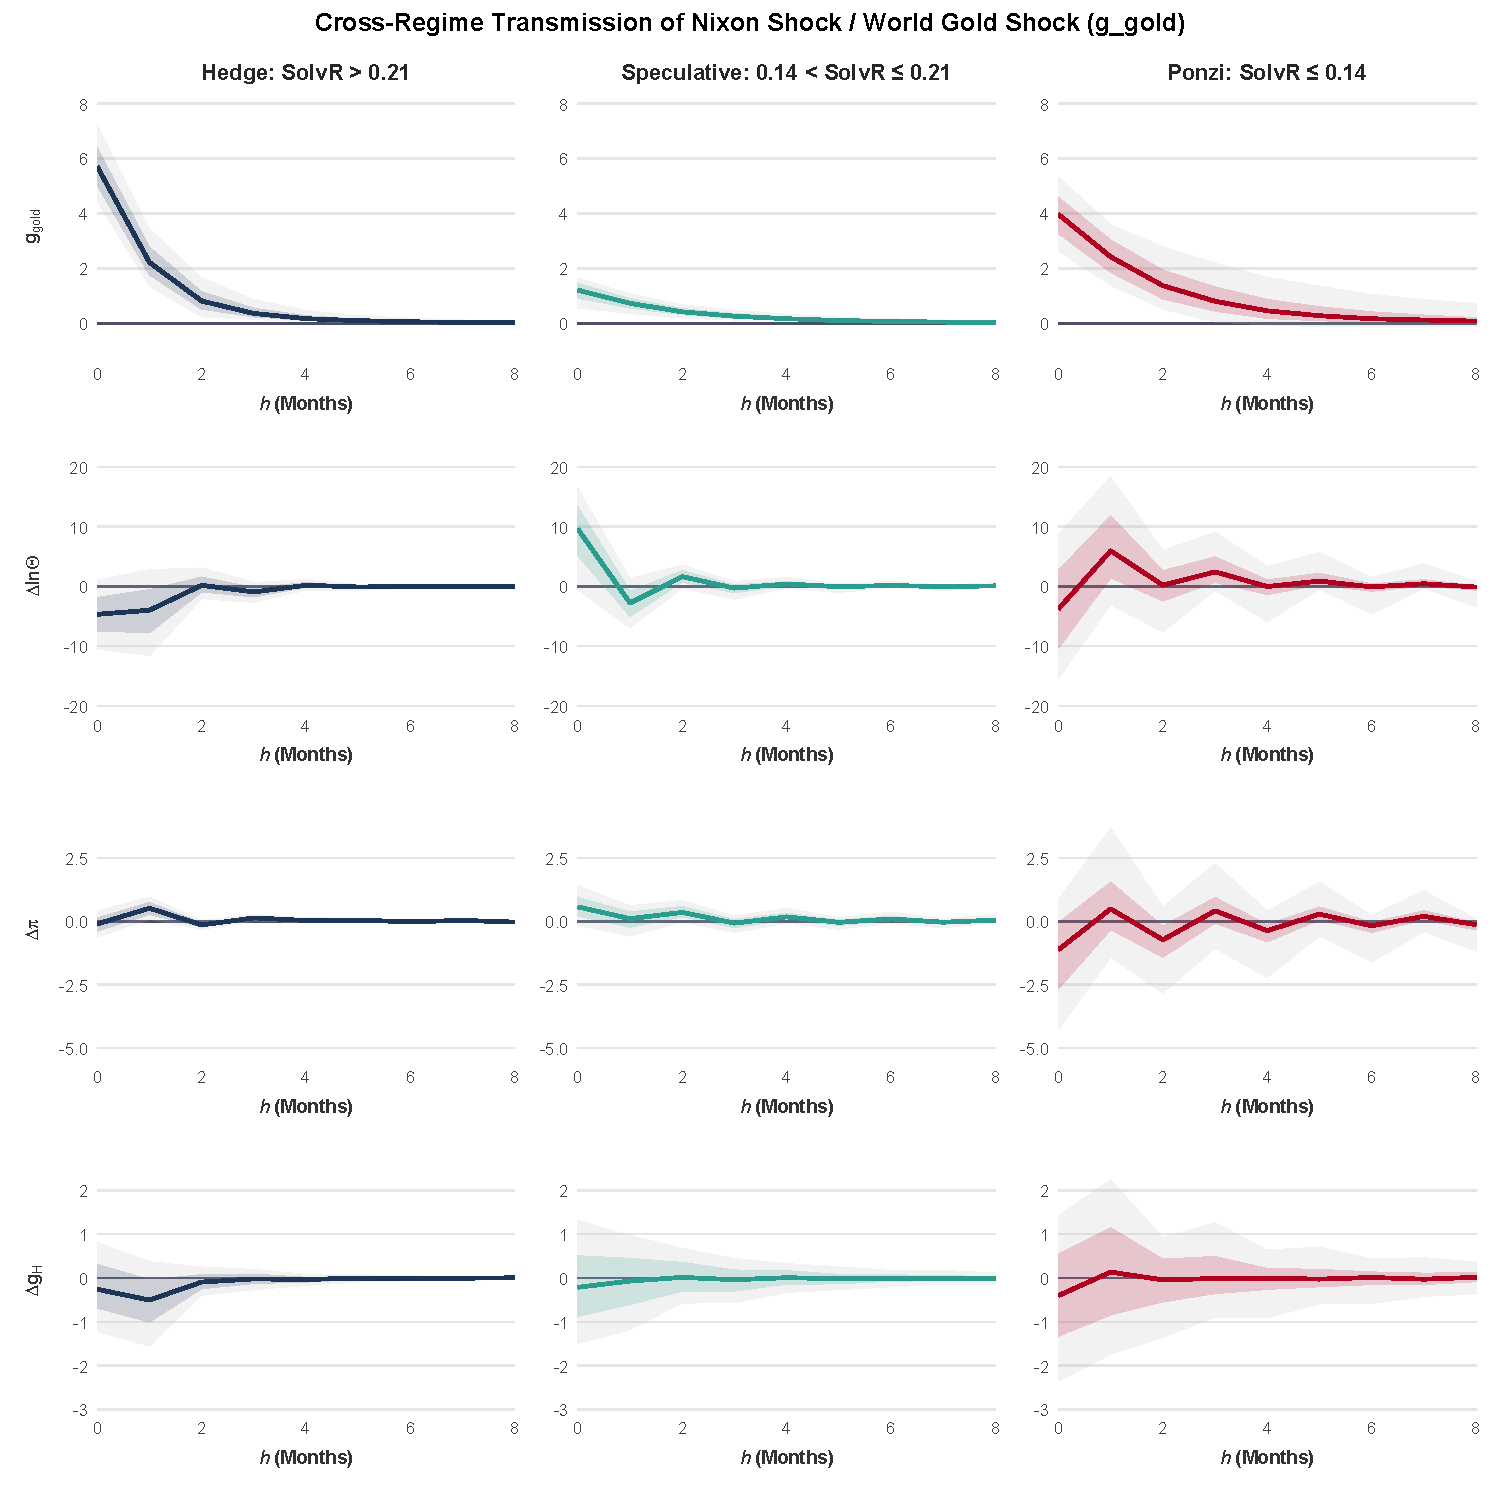
\includegraphics[width=0.92\textwidth]{figures/fig_app_c04_gold_shock_atlas.pdf}
\begin{tabular}{p{0.95\textwidth}}
\footnotesize \textbf{Notes:} Comparative cross-regime Generalized Impulse Response Functions (GIRF) to a $+1\sigma$ international gold price growth shock ($g_{P,\text{gold}}$) across Hedge ($\text{SolvR} > 0.21$, solid navy line), Speculative ($0.14 < \text{SolvR} \le 0.21$, dashed gold line), and Forced Ponzi ($\text{SolvR} \le 0.14$, dotted crimson line) regimes from the 3-regime TVAR(1) ($d=1$). Structural identification follows the recursive Cholesky ordering vector $[g_{P,\text{gold},t}, \Delta \ln \Theta_t, \Delta \pi_t, \Delta g_{H,t}]'$ certified by the PCMCI DAG. Shaded areas represent 68\% and 95\% stratified residual bootstrap bands ($B=500$) across horizon $h=0\dots 8$ months, evaluated against the neutral grey horizontal zero reference line. Responses are expressed in percentage-point monthly deviations. World-money stagflation transmits into severe domestic cost wedges only when the Central Bank lacks foreign reserve cushions. Data sources: London Bullion Market, Central Bank of Chile, and INE (1960:01--1980:12).
\end{tabular}
\end{figure}

\begin{figure}[H]
\centering
\caption{Cross-Regime Transmission Atlas: Real Structural Imbalance Shock ($\Delta \ln \Theta$)}
\label{fig:app_c05_scissors_atlas}
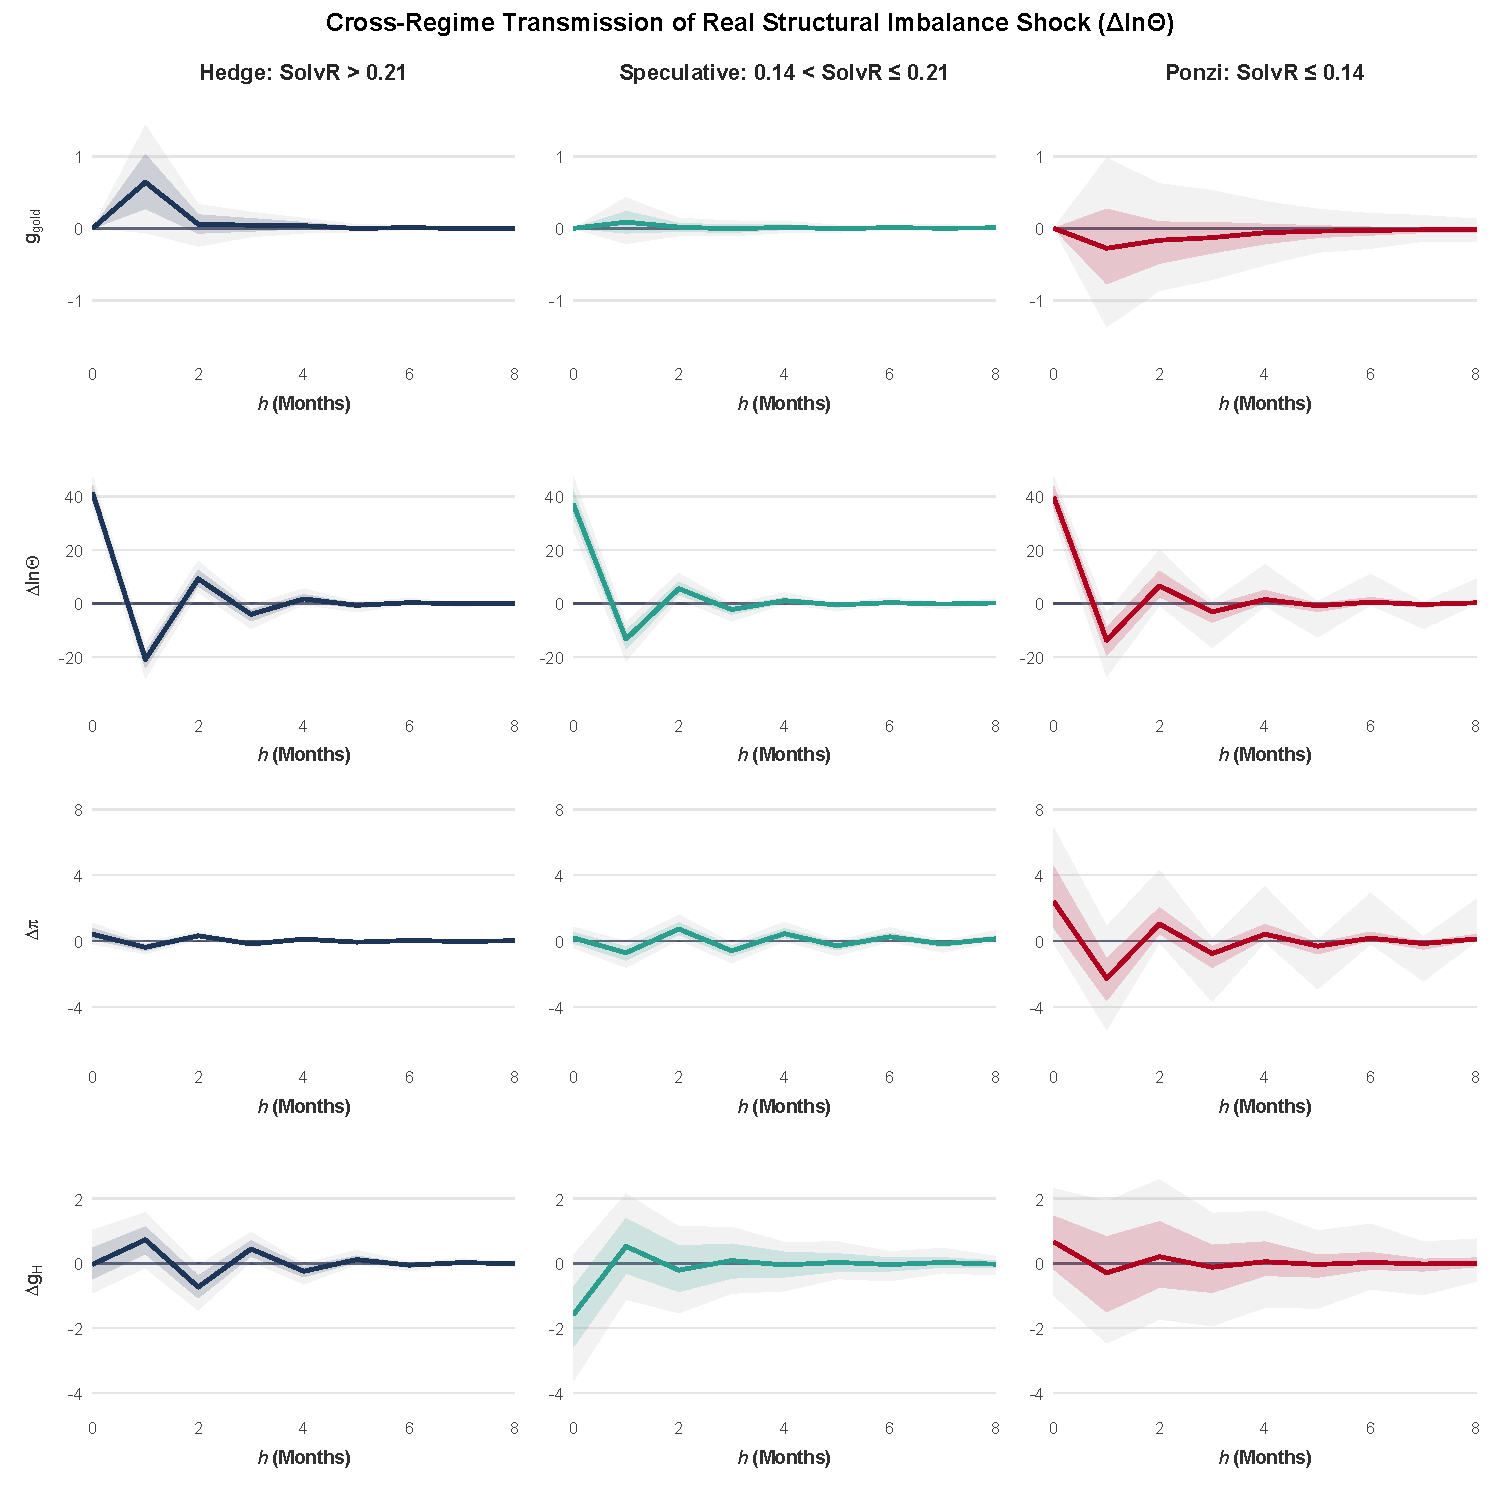
\includegraphics[width=0.92\textwidth]{figures/fig_app_c05_scissors_shock_atlas.pdf}
\begin{tabular}{p{0.95\textwidth}}
\footnotesize \textbf{Notes:} Comparative cross-regime Generalized Impulse Response Functions (GIRF) to a $+1\sigma$ Real Structural Imbalance shock ($\Delta \ln \Theta$) across Hedge ($\text{SolvR} > 0.21$, solid navy line), Speculative ($0.14 < \text{SolvR} \le 0.21$, dashed gold line), and Forced Ponzi ($\text{SolvR} \le 0.14$, dotted crimson line) regimes from the 3-regime TVAR(1) ($d=1$). Structural identification follows the recursive Cholesky vector $[g_{P,\text{gold},t}, \Delta \ln \Theta_t, \Delta \pi_t, \Delta g_{H,t}]'$ certified by the PCMCI DAG. Shaded ribbons depict 68\% and 95\% stratified residual bootstrap credibility bands ($B=500$) across $h=0\dots 8$ months, evaluated against the neutral grey horizontal zero reference line. Responses are in percentage-point monthly deviations. Import asphyxiation triggers immediate output contraction and explosive inflation jumps under balance-sheet insolvency. Data sources: Central Bank of Chile (BCCh) and INE (1960:01--1980:12).
\end{tabular}
\end{figure}